% !TeX root = ../sustechthesis-example.tex

\chapter{部分基本固件设计实现图和激光幅度稳定拓展方案图}

\begin{figure}
    \centering
    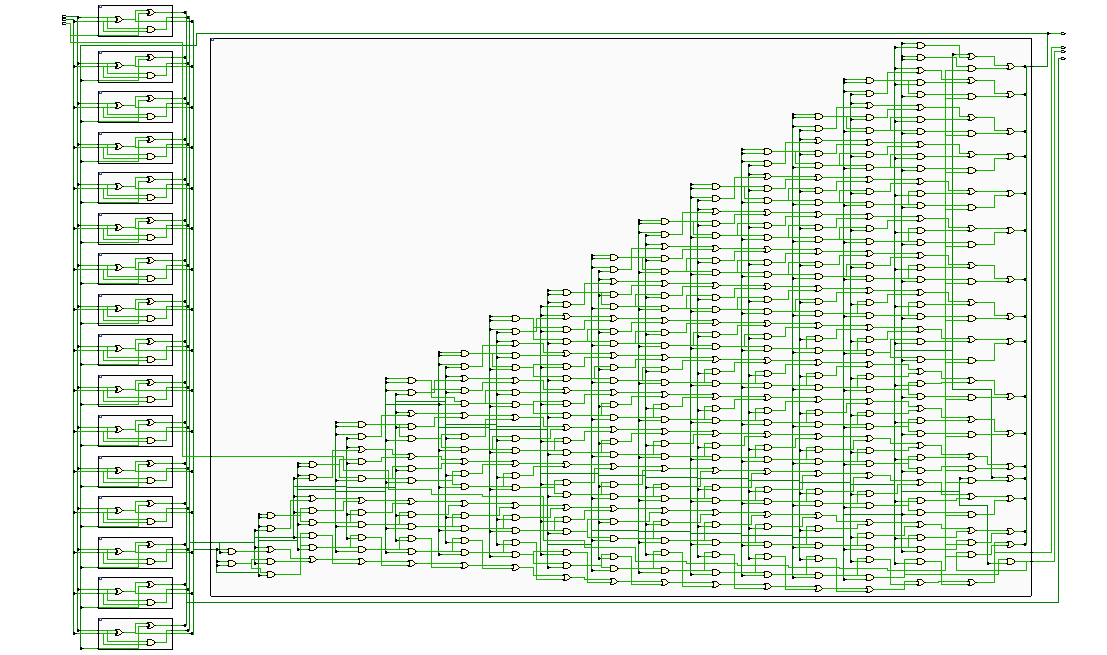
\includegraphics[width=1.0\linewidth]{rtmq/ahead_adder_16bits}
    \caption[16位超前进位加法器的FPGA实现结构图]{16位超前进位加法器的FPGA实现结构图(Vivado)\label{fig:ahead_adder_16bits}}
\end{figure}


\begin{figure}
    \centering
    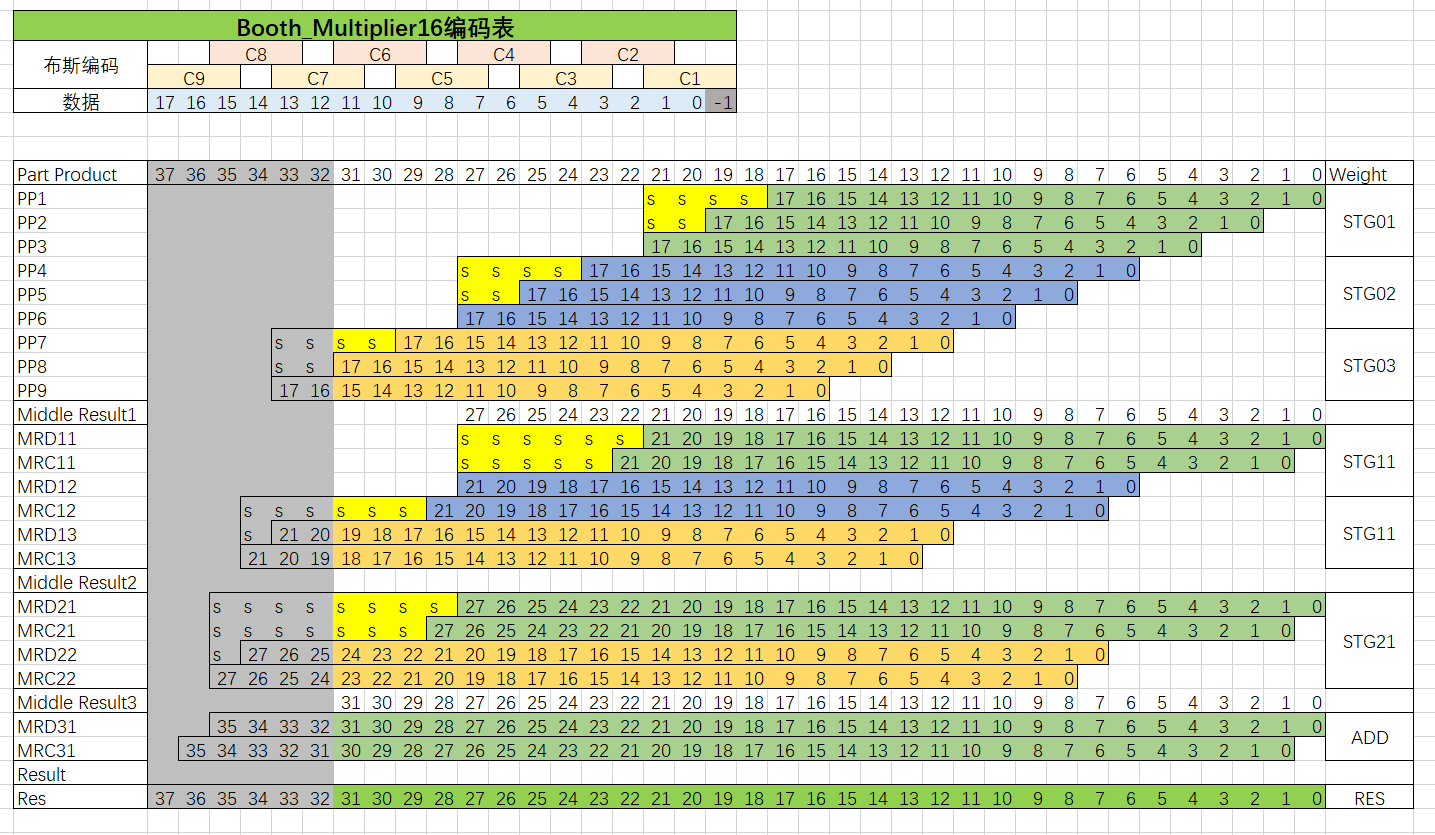
\includegraphics[width=1.0\linewidth]{rtmq/booth_multiplier_16bits_basic}
    \caption[16位Booth乘法器编码和加法树表]{16位Booth乘法器编码和加法树表\label{fig:booth_multiplier_32bits_basic}}
\end{figure}

\begin{figure}
    \centering
    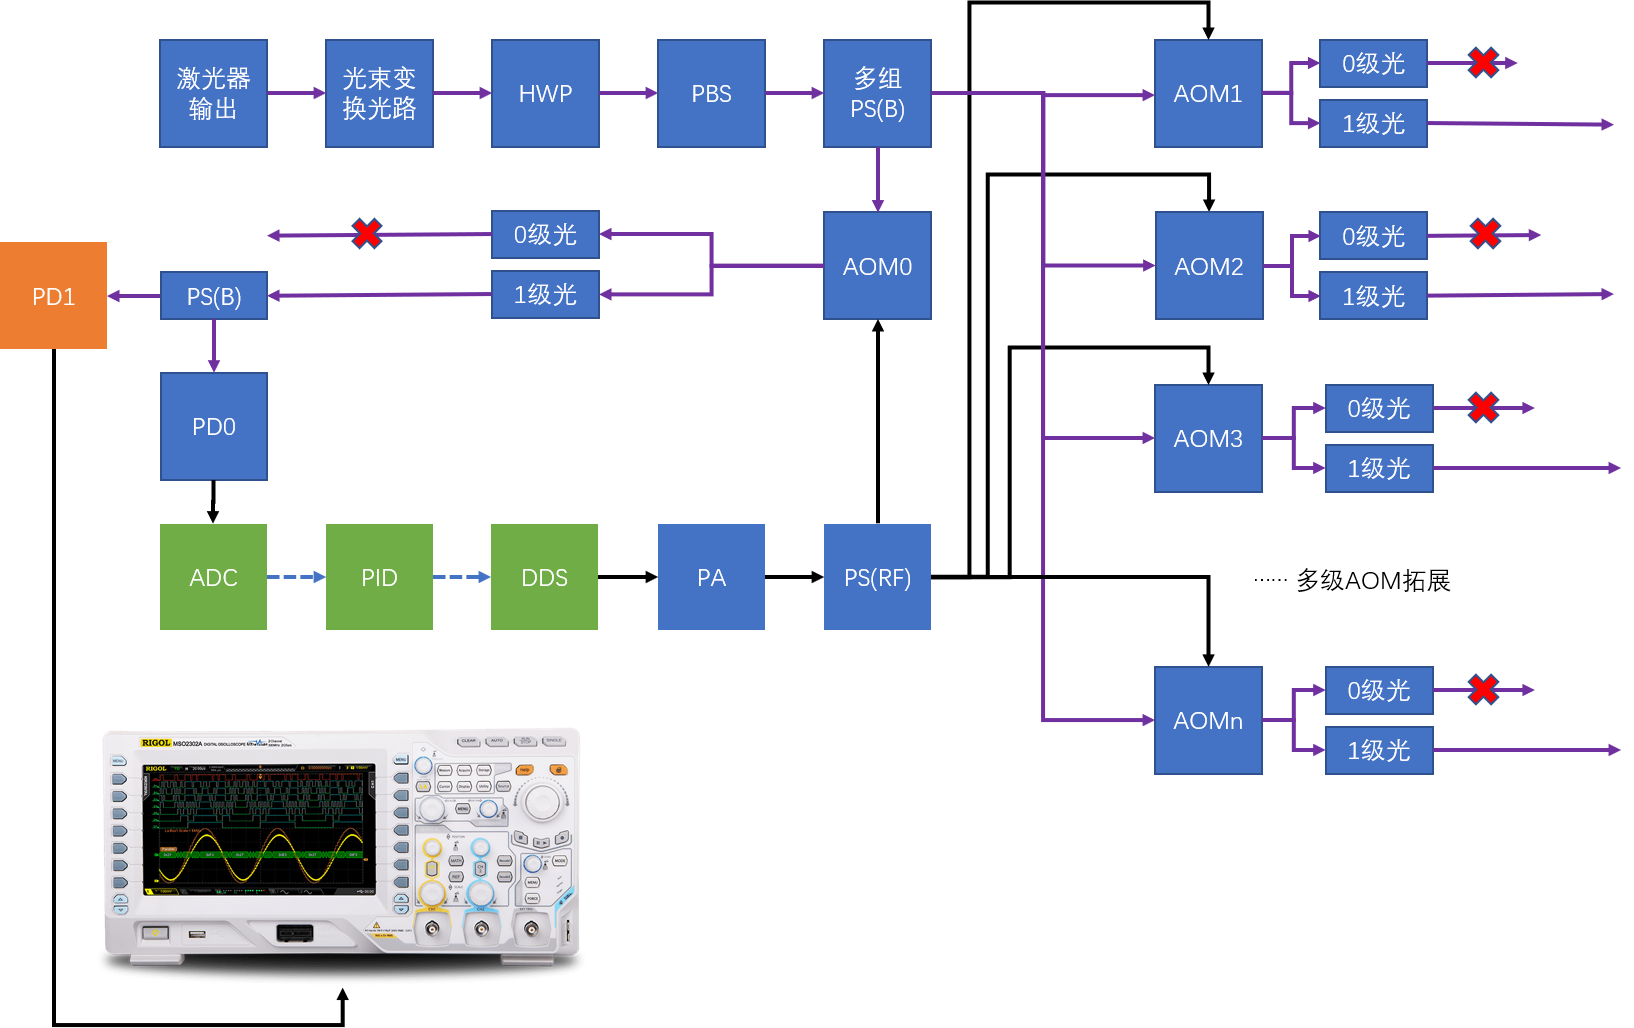
\includegraphics[width=1.0\linewidth]{laser_stabilization1}
    \caption[激光幅度外部稳定的拓展方案架构图]{激光幅度外部稳定的拓展方案架构图\label{fig:laser_stabilization}}
\end{figure}

% \begin{figure}
%     \centering
%     \caption[实验室中实际离子阱系统图]{实验室中实际离子阱系统图\label{fig:ion_trap_system}}
%     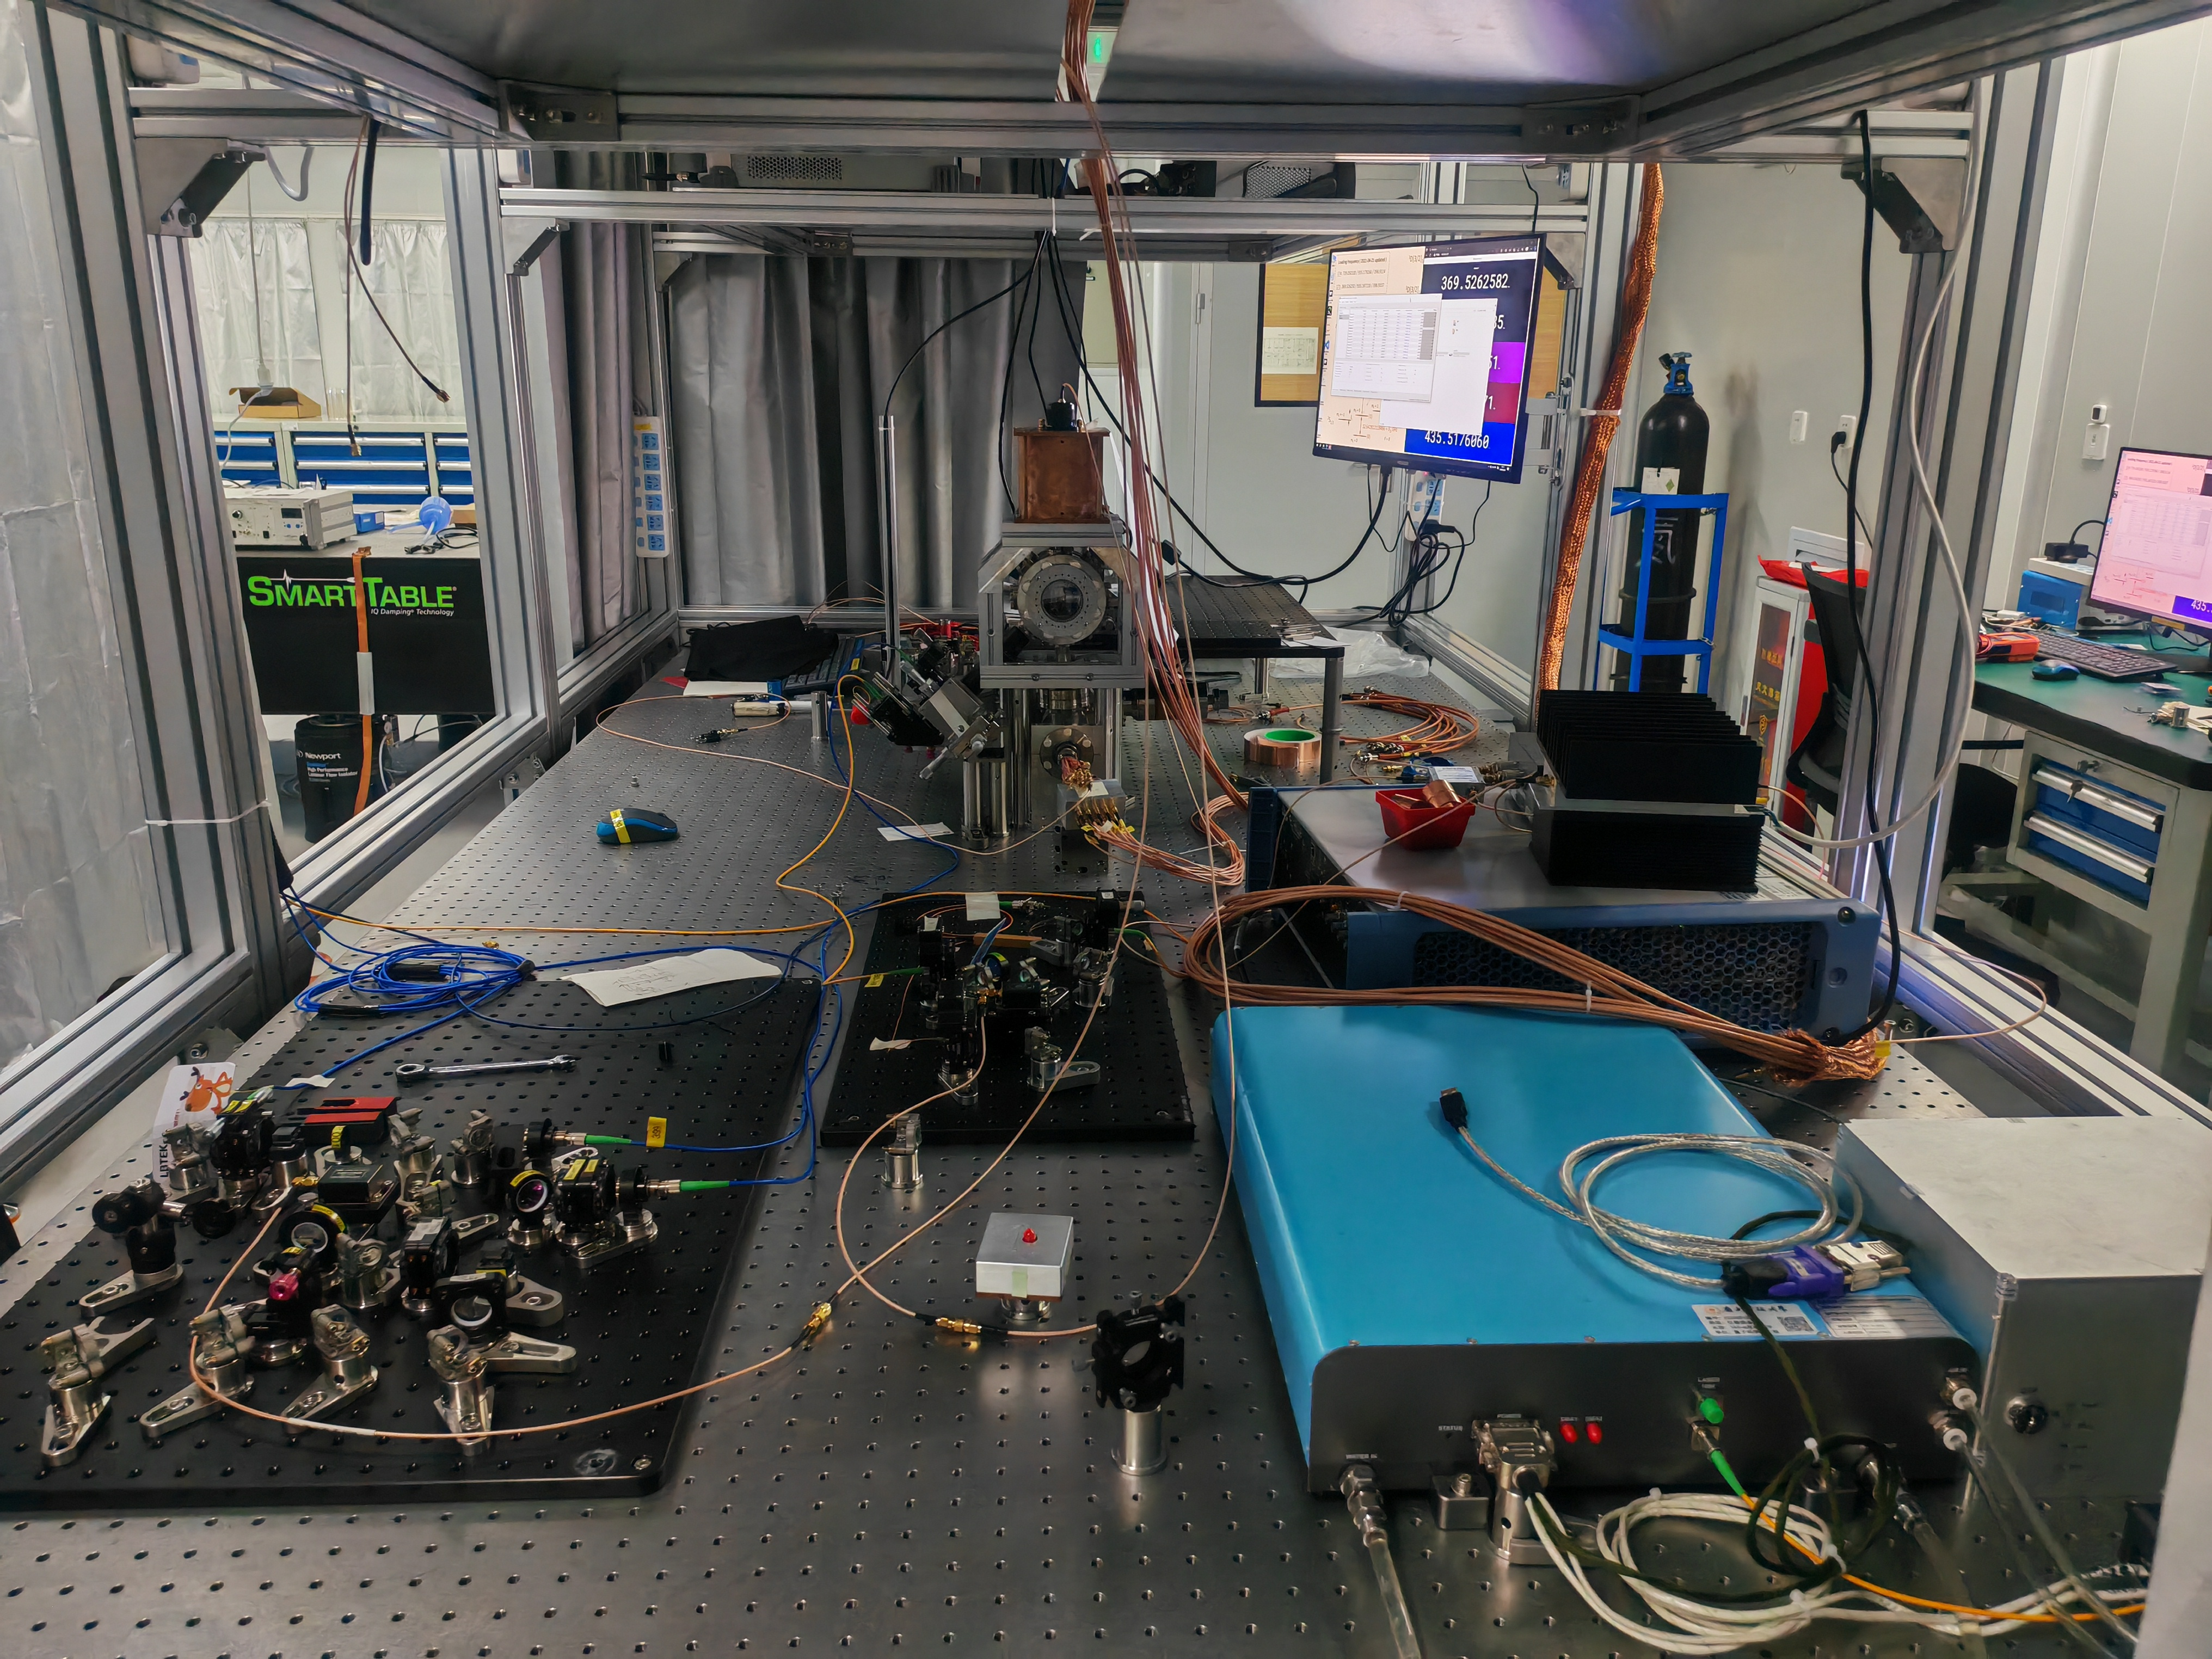
\includegraphics[width=1.0\linewidth]{ion_trap_system}
% \end{figure}